\documentclass{article}

\usepackage[mathcal,mathbf]{euler}
\usepackage{theorem,amsmath,enumerate,fancyhdr,amssymb,amsfonts}
\usepackage[pdftex]{graphicx}
\usepackage{algorithm}
\usepackage{algorithmic}

\usepackage{myDefs}
\usepackage{undertilde}
\usepackage{diagbox}

\title{ 
    Algorithmic Learning Theory\\
    Spring 2017\\
    Lecture 5
}

\author{
    {\bf Instructor:} Farid Alizadeh\\
    {\bf Scribe:} Weiting Gao\\
}

\date{02/15/2017}

\begin{document}

\pagestyle{fancy}

\lhead{
    {\bf Scribe: }{Weiting Gao }\\
    {\bf Lecture 5}
}

\rhead{
    {\bf Date: }{02/15/2017}
}

\maketitle

\medskip

This lecture introduces tree partitioning algorithm and naive Bayes method, and discusses the following:
\begin{enumerate}
	\item Tree Partitioning Algorithm
	\begin{enumerate}
		\item Application of Tree Partitioning Algorithm
		\item Tree-based Partition and k-NN
		\item Tree Partitioning Algorithm
		\item Issues with Splitting
		\item Stopping Criteria
	\end{enumerate}
	\item The Naive Bayes Method
\end{enumerate}

\clearpage

\section{Tree Partitioning Algorithm}{
	 The tree algorithm is a form of partitioning that the partitioning boundaries are parallel to the axis. And one advantage of this type of partitioning is that you can immediately associate it with a decision tree.
	
	 To see how it works, we suppose there are two features $x_1$ and $x_2$. We assume that there is an upper limit for all feature, so the whole universe is inside the giant hyperrectangle. The following graph shows the partition.
	 \begin{center}
		 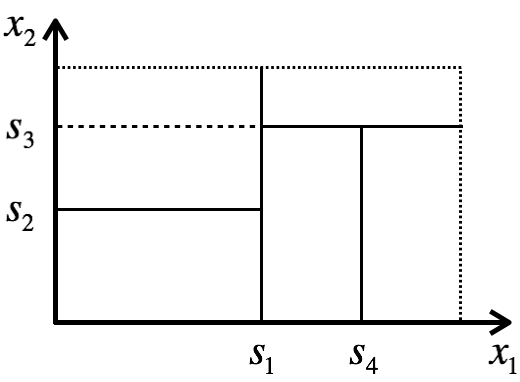
\includegraphics[scale=0.65]{images/Rectangle.png}
		 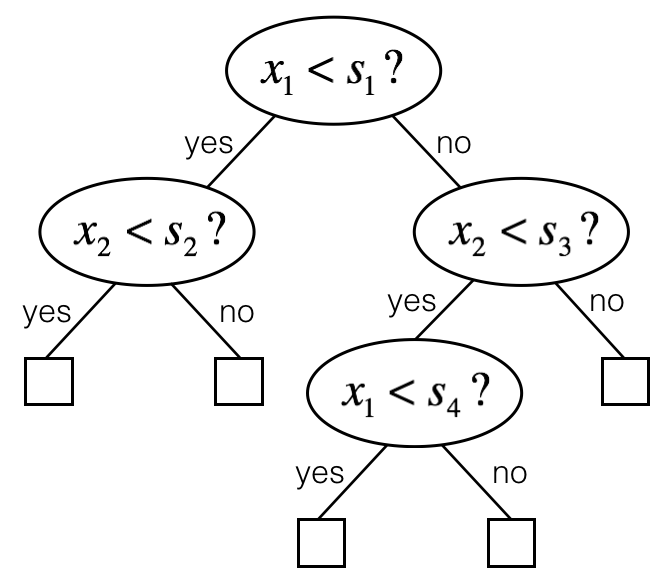
\includegraphics[scale=0.5]{images/DecisionTree.png}
	 \end{center}  
	 Without any partitioning, the entire feature space is one region, which is the root node in the decision tree. If we decide to split on the $x_1$ at the point $s_1$, we split at $x_1$ along the vertical line, which corresponds to the question that whether $x_1$ is less than $s_1$. If the answer is yes, the new point goes to the left of $x_1=s_1$ and to the right otherwise.
	 
	 The next step we have two regions that we can decide.Also, we should decide which coordinate to split. If we decide to split on the $x_2$ at $s_2$, we split at $x_2$ along the horizontal line from $s_2$. The corresponding question is whether $x_2$ is less than $s_2$. If the answer is yes, the new point goes to the lower rectangle and to the higher rectangle otherwise. And the process goes on as this rule. 
	 
\subsection{Application of Tree Partitioning Algorithm}{
	The advantage of this partitioning is that it gives you a decision tree, so every region corresponds to a terminal node or leaf. And in this leaf, we can trace back, so the sequence of questions that let us to this point is given. 
	
	In practical situation, it is a very attractive algorithm because it corresponds to a decision tree. 
	 
	For example, if you look at whether to approve credit for someone or not. Such a decision tree may help make decisions  according to several questions answered by customers. At least you can see why credit was not approved because we can see the sequence of questions.}

\subsection{Tree-based Partition and k-NN}{
	Tree partitioning is a special case of partition where all the lines are parallel to the axis and all the regions are rectangular. And it is similar in some sense to the k-NN except the neighborhood is replaced by the rectangle in which the point falls. If a new point comes in, we find out the rectangle and consider it as a surrogate to the neighborhood. It is a different mechanism to come up with the neighborhood.
	
	So, the statistic justification is very similar to k-NN. We should calculate  \(P_r[y|x]\). In k-NN, $x$ is the $k$ nearest neighbors of the new point. However, in tree partitioning algorithm, $x$ is replaced by the rectangle where $x$ falls in. And \(P_r[y|x]\) is approximate to the average over training set $y$ of points falling in the rectangle. For numerical problem, it would be the average of $y$ of all points that fall in this rectangle. For categorical problem, it would be the majority class in this rectangle.
}
	
\subsection{Tree Partitioning Algorithm}
 Supposed that we have a data set as follows:
	
     \begin{center}{
	 		\begin{tabular}{c|c c c c }
	 			
	 			$y$ & $x_1$ & $x_2$ & ... & $x_p$ \\
	 			\hline
	 			$y_1$ & $x_{11}$ & $x_{12}$ & ... & $x_{1p}$ \\
	 			
	 			$y_2$ & $x_{21}$ & $x_{22}$ & ... & $x_{2p}$ \\
	 			
	 			... & ...  ... & ... & ... \\
	 			
	 			$y_n$ & $x_{n1}$ & $x_{n2}$ & ... & $x_{np}$ \\
	 			
	 		\end{tabular}
	 	}
	 \end{center}
	 
	 Given the data, in the feature space, there are $n$ points, and we should partition them into a number of regions. However, the total number of partition is extremely large and we can not calculate it. Bell Numbers($B_n$), is the number of partitions of a set of $n$ elements. 
	 
	 Finding the best partition is an NP-hard problem, meaning that there is not a good algorithm for it. So you can just go over all the possible partitions and evaluate the quality of each one, choose the best. Also, if we want to find the best decision tree, we should think of all possible decisions trees that can be constructed from data even if they are large.
	 
	 So we use greedy algorithm, which is suboptimal.  Although it does not guarantee to give best decision variable, it can at least evaluate this quality.
	 
	 Now we know the way to find the best partition. In addition, we should also notice that at each iteration, three things should be decided:
	 
	 \begin{enumerate}
	 	\item which region to split
	 	\item which coordinate to split
	 	\item the location to split
	 \end{enumerate}


     The algorithm is as follows:
     
     \begin{algorithm}
     	\caption{Best tree splitting}
     	\label{alg1}
     	\begin{algorithmic}
     		\REQUIRE P(features) K(regions)
     		\ENSURE S
     		\FOR{$K=1$ to $k$} 
     		\STATE
     		\FOR{$i=1$ to $P$}
     		\STATE $i_k\rightarrow \text{region}K,\text{feature}x_i$
     	
     		\ENDFOR 
     		\ENDFOR
     		\STATE find best $S$
     	\end{algorithmic}
     \end{algorithm}
     
\subsection{Issues with Splitting}

There are four cases of splitting:

  \begin{center}{
 		\begin{tabular}{c|c c}
 			
 			\diagbox{$y$}{$x_i$} & numerical & categorical\\
 			\hline
 			numerical & ($x_i$:numerical $y$:numerical) & ($x
 			_i$:categorical $y$:numerical) \\
 			
 			categorical & ($x_i$:numerical $y$:categorical) & ($x_i$:categorical $y$:categorical)\\
 			
 			
 		\end{tabular}
 	}
 \end{center}	}
\subsubsection{
$x_i$-numerical $y$-numerical}
	Suppose $x_i$ and $y$ are both numerical and their values are as follows:
	\[x_i=\{1,2,5,7\}\]
\[y=\{7,6,8,3\}\]	
Here are three possible splits and the corresponding square loss:
\begin{enumerate}
	\item \[x_i:(1)(2,5,7)\]
	\[y:(7)(6,8,3)\]

	(7) $\rightarrow$ \(\text{square loss}=0\)

(6,8,3) $\rightarrow$ \(\text{average of y}=\frac{6+8+3}{3}=5.67\)

\medspace \(\text{square loss}=(6-5.67)^2+(8-5.67)^2+(3-5.67)^2=12.67\)
 
 total square loss: \(0+12.67=12.67\)
 
 \item \[x_i:(1,2)(5,7)\]
 \[y:(7,6)(8,3)\]
 	(7,6) $\rightarrow$  \(\text{average of y}=\frac{7+6}{2}=6.5\)
 	 \(\text{square loss}=(7-6.5)^2+(6-6.5)^2=0.5\)
 	
 	(6,8,3) $\rightarrow$ \(\text{average of y}=\frac{8+3}{2}=5.5\)
 	
 	\(\text{square loss}=(8-5.5)^2+(3-5.5)^2=12.5\)
 	
 	total square loss: \(0.5+12.5=13\)
 	
 \item \[x_i:(1,2,5)(7)\]
 \[y:(7,6,8)(3)\]
 (7,6,8) $\rightarrow$  \(\text{average of y}=\frac{7+6+8}{3}=7\)
 
 \(\text{square loss}=(7-7)^2+(6-7)^2+(8-7)^2=2\)
 
 (3) $\rightarrow$ \(\text{square loss}=0\)
 
 total square loss:\(2+0=2\)
 
 \medskip
 The total square loss of the third partition is smallest, so $(1,2,5)(7)$ is the best partition.

\end{enumerate}

\subsubsection{$x_i$-numerical $y$-categorical}
Suppose we have
\[x_i:(2,4,6)\]
\[y:\text{two classes: red, blue}\]

 \begin{center}
 	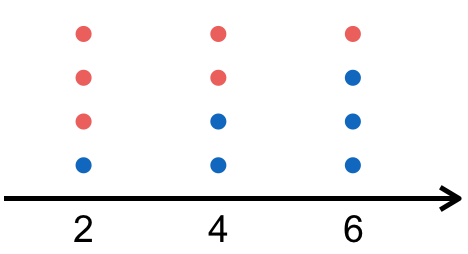
\includegraphics[scale=0.65]{images/numerical.png}
 
 \end{center}  
We compare the misclassification rate before and after splitting.

Before we split  $\rightarrow$ \(\text{misclassification rate}=\frac{6}{12}\)

Here are two possible splits:

\begin{enumerate}
	\item  \[x_i:(2)(4,6)\]
	(2) $\rightarrow$ \(\text{misclassification rate}=\frac{1}{4}\)
	
	(4,6) $\rightarrow$ \(\text{misclassification rate}=\frac{3}{8}\)
	
	total misclassification rate: \(\frac{4}{12}\times\frac{1}{4}+\frac{8}{12}\times\frac{3}{8}=\frac{4}{12}\)
	
	\item  \[x_i:(2,4)(6)\] 
	(2,4) $\rightarrow$ \(\text{misclassification rate}=\frac{3}{8}\)
	
	(4,6) $\rightarrow$ \(\text{misclassification rate}=\frac{1}{4}\)
	
	total misclassification rate: \(\frac{4}{12}\times\frac{1}{4}+\frac{8}{12}\times\frac{3}{8}=\frac{4}{12}\)
\end{enumerate}

We reduce the misclassification rate from $\frac{6}{12}$ to $\frac{4}{12}$ by splitting. However the misclassification of two splits are same. We can not find which split is better according to misclassification rate. 

Actually, misclassification rate is not a good measure to evaluate the partition. Here we introduce $\text{Cross Entropy}$ and $\text{Gini Index}$, which are preferable to misclassification rate. 
For a two-class problem, suppose the proportion of of items in $class1$ and $class2$ are $p$ and $1-p$. 

The entropy in this case is defined as \[\text{entropy}=H(p)=-p\mathit{log}p-(1-p)\mathit{log}(1-p)\]
 
\(\text{where the logarithm is usually in base 2 and }  0\mathit{log}0=0\)

\medskip
The Gini index is defined as \[\text{Gini index}=G(p)=2 p(1-p)\]

Misclassification rate is defined as \[\text{misclassification rate}=E(p)=1-\mathit{max}(p,1-p)\]
These three measures are shown in the following graph:
\begin{center}
	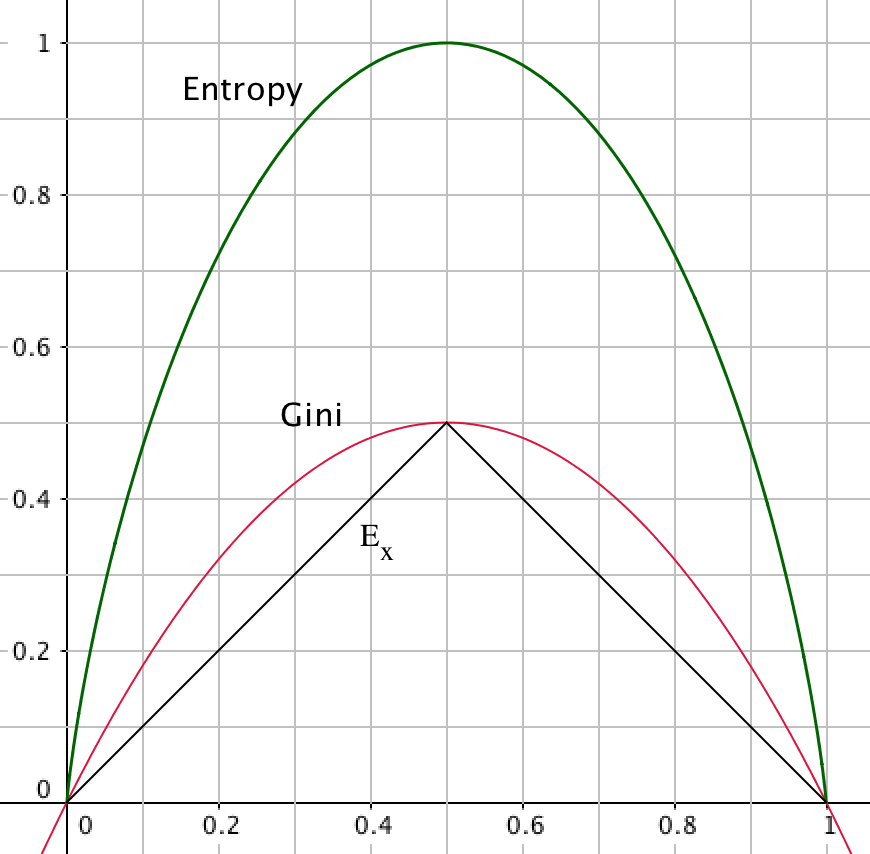
\includegraphics[scale=0.55]{images/Gini1.png}
	
\end{center}  


\paragraph{eg.}{
Suppose we have 8 points, in which 7 of them are blue and 1 of them is red. And we split in the middle. The figure is shown as follows:
 \begin{center}
 	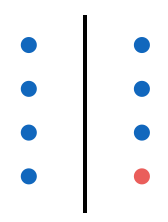
\includegraphics[scale=0.65]{images/split.png}
 \end{center}  

Now, we calculate the $\text{misclassification rate}$, $\text{cross entropy}$ and $\text{Gini index}$ before and after split.

Before split:\[\text{misclassification rate}=0.125\]
\[\text{Entropy}=-\frac{1}{8}\mathit{log}\frac{1}{8}-\frac{7}{8}\mathit{log}\frac{7}{8}\approx0.544\]
\[\text{Gini index}=2\times\frac{1}{8}\times\frac{7}{8}\approx0.219\]

After split:\[\text{misclassification rate}=0.125\]
\[\text{Entropy}=\frac{1}{2}\times0+\frac{1}{2}\times(-\mathit{log}\frac{1}{4}-\frac{3}{4}\mathit{log}\frac{3}{4})=0.405\] 
\[\text{Gini index}=\frac{1}{2}\times0+\frac{1}{2}\times2\times\frac{3}{4}\times\frac{1}{4}=0.1875\]

As we can see, after splitting, both $\text{entropy}$ and $\text{Gini index}$ reduce. However, the misclassification rate remains the same, which means this split is useless and it did not make any difference. 

But the split is actually very informative. Before the split, when the new point comes in, we estimate that there is $\frac{1}{8}$ chance of making an error. After the split, the point must be blue if it goes to the left side. On the other hand, there is $\frac{3}{4}$ chance of being blue if it goes to the right side, which may result in further splitting. Misclassification rate can not show this information but either $\text{Gini index}$ or $\text{entropy}$ would distinguish. This is why the misclassification rate is not a good measure. So, we use $\text{Gini index}$ or $\text{entropy}$ to test the quality of partition.

\subsubsection{$x_i$-categorical $y$-numerical}
Suppose we have $x_i$ and $y$ as follows:
	\[x_i=\{a,b,c,d\}\]
	\[y=\{7,6,8,3\}\]	
	Here are $7$ possible splits:

\begin{enumerate}
	\item \((a)(b,c,d)\)
	\item \((b)(a,c,d)\)
	\item \((c)(a,b,d)\)
    \item \((d)(a,b,c)\)
    \item \((a,b)(c,d)\)
    \item \((a,c)(b,d)\)
    \item \((a,d)(b,c)\)
	
\end{enumerate}

Notice that when $x_i$ is categorical, it does not have order, which is different from the situation when $x_i$ is numerical. Actually, if we consider the categorical variable with $k$ level, there are \(2^{k-1}-1\) different ways to split the features into 2 subsets.

After decide the possible splits, the following process is actually same with the situation where both $x_i$ and $y$ are numerical. We should then calculate the square loss of each partition and choose the partition whose square loss is smallest.

\subsubsection{$x_i$-categorical $y$-categorical}{
	Suppose we have
	\[x_i:(a,b,c)\]
	\[y:\text{two classes: red, blue}\]
	 \begin{center}
	 	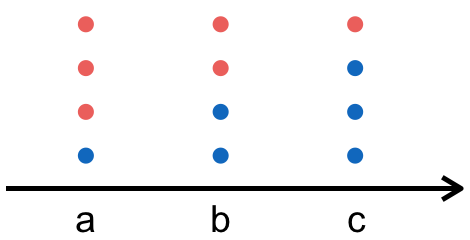
\includegraphics[scale=0.65]{images/categorical.png}
	 \end{center}  
	
	We compare the misclassification rate before and after splitting.
	
	Before we split  $\rightarrow$ \(\text{misclassification rate}=\frac{6}{12}\)
	
	Here are three possible splits:
	
	\begin{enumerate}
		\item  \[x_i:(a)(b,c)\]
		(a) $\rightarrow$ \(\text{misclassification rate}=\frac{1}{4}\)
		
		(b,c) $\rightarrow$ \(\text{misclassification rate}=\frac{3}{8}\)
		
		total misclassification rate: \(\frac{4}{12}\times\frac{1}{4}+\frac{8}{12}\times\frac{3}{8}=\frac{4}{12}\)
		
		\item  \[x_i:(b)(a,c)\] 
		(b) $\rightarrow$ \(\text{misclassification rate}=\frac{1}{2}\)
		
		(a,c) $\rightarrow$ \(\text{misclassification rate}=\frac{1}{2}\)
		
		total misclassification rate: \(\frac{4}{12}\times\frac{1}{2}+\frac{8}{12}\times\frac{1}{2}=\frac{6}{12}\)
		
		\item  \[x_i:(c)(a,b)\] 
		(c) $\rightarrow$ \(\text{misclassification rate}=\frac{1}{4}\)
		
		(a,b) $\rightarrow$ \(\text{misclassification rate}=\frac{3}{8}\)
		
		total misclassification rate: \(\frac{4}{12}\times\frac{1}{4}+\frac{8}{12}\times\frac{3}{8}=\frac{4}{12}\)
	\end{enumerate}
	
	The best partition in this case is $(a)(b,c)$ or $(c)(a,b)$. We reduce the misclassification rate from $\frac{6}{12}$ to $\frac{4}{12}$ by splitting.

\subsection{Stopping Criteria}
 Suppose we have $n$ data points, we use the size of tree $|T|$ to be the number of leaves, which is same with the number of split regions. This is measure of the complexity of the model. If the region only contains a small number of data points, the process will stop when the leaves of the tree contain only one data point. However, imagine we have thousands of data points, it would be costly if we go all the ways and make every leaf contains only one point. Also, it will lead to overfitting since the data will make zero error. 
	
	Unlike k-NN in which we should test all possible $k$ and choose the best one, when we build tree, even if we fix the number of leaves, there still exists many kinds of decision trees which contain equal number of leaves. Also, when the number of leaves goes large, the types of trees will be extremely large. So we can not just change the number of leaves, the method is following.
	
	So far we use the loss function to evaluate the tree, now we add $\alpha|T|$. So the we modify "loss function" to \[\mathit{loss}(T)+\alpha|T|\] 
where $\alpha$ is a fixed constant.

Every time you make a split, one more leaf is added, you reduce $\mathit{loss}(T)$ but you increase $\alpha|T|$. If the split result in the reduction of $\mathit{loss}(T)$ is more than increase of $\alpha|T|$, the total number will reduce, otherwise the total number will increase. So this algorithm is that you set $\alpha|T|$, then keep splitting until no split can reduce the total number.

The problem is that if we do base on this algorithm, we may not catch some stage that have sudden reduction. Here is one example.

 \begin{center}
 	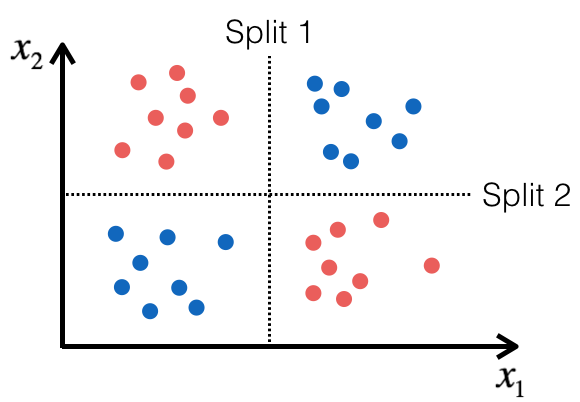
\includegraphics[scale=0.65]{images/2split.png}
 \end{center}  

In this example, the first split only makes very marginal improvement. If we use this stopping criteria, we may stop splitting before this split since it cannot reduce the total number \(\mathit{loss}(T)+\alpha|T|\). But if we keep doing the second split, there will be a sudden reduction of the total number and each region will be pure, which is excellent. As we can see, this stopping criteria could miss things like this.

We can use another method to avoid this problem. You go all the ways to build the tree to the fullest extension, and then go backwards by taking two sibling leaves and merging them. When you merge, the  $\mathit{loss}(T)$ will increase, in each stage find two nodes that cause the least amount of increase. In this way, you build the sequence of tree backwards until it has only one node. And in this sequence, you find the best tree.

 \begin{center}
 	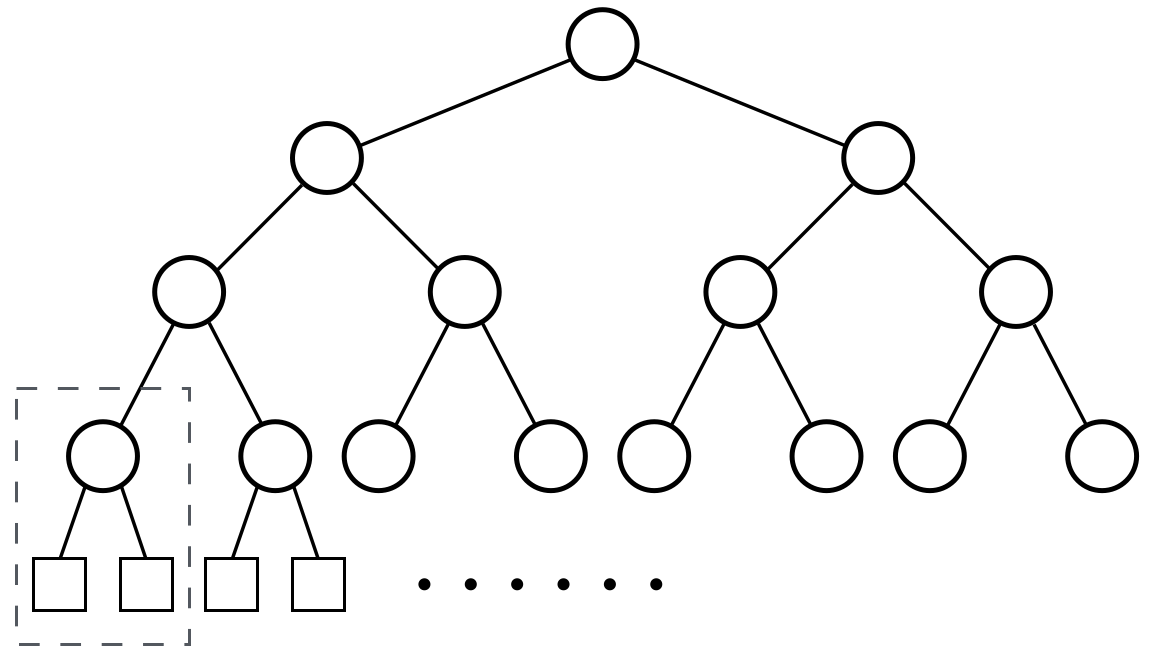
\includegraphics[scale=0.45]{images/BackwardTree.png}
 \end{center}  
 
\section{The Naive Bayes Method}{
	The Bayes formula:	\[\mathit{f}(y|\utilde{x})=\frac{\mathit{f}(\utilde{x}|y)\mathit{f}(y)}{\mathit{f}(\utilde{x})}\]
	
	It is not possible to compute the value, we can only estimate it.
	In the process of tree partitioning and k-NN, they approximate $\mathit{f}(y|\utilde{x})$ by replacing the particular $x$ with neighborhood or region. Then estimate the distribution of $y$. If $y$ is categorical, calculate the percentage of each class.
	
	Now consider the classification situation.
	The Bayes formula:
	
	\[\mathit{y} \in \{1,2,\cdots ,k\}\]
	
	\[Pr[y=i|\utilde{x}]=\frac{\mathit{f}(\utilde{x}|y=i)Pr[y=i]}{\mathit{f}(\utilde{x})}, i=1,2,\cdots ,k\]

	For each $y$, the denominator is same. So when finding the largest $y$, we can ignore the denominator. In addition, we can compute or estimate $Pr[y=i]$ since it does not depend on $x$. So we can only focus on the joint density \(Pr[y=i|\utilde{x}]\). If we can compute this, find the distribution of $x$ for each level, then the problem is solved.
	
	The most important part of Naive Bayes is that it make an assumption that features $x_1,x_2,\cdots,x_p$ are independent, so
	\[\mathit{f}_i(x)=\mathit{f}_i(x_1)\mathit{f}_i(x_2)\cdots \mathit{f}_i(x_p)\]
	
	Therefore we can concentrate on each feature alone, estimate probabilities, and multiply them to get the joint probability.
	
\paragraph{eg.}
If $y$ is credit approved or not approved, and $x_i$ are the features of the customers. $x_1=\text{income}$, $x_2=\text{age}$, $x_3=\text{marital status}$

We calculate the joint distribution of income, age and marital status given credit approved or rejected.
	\[\mathit{f}(\text{income, age, marital status}\,|\,+)=f_{+}(\text{income})f_{+}(\text{age})f_{+}(\text{marital status})\]
	
	\[\mathit{f}(\text{income, age, marital status}\,|\,-)=f_{-}(\text{income})f_{-}(\text{age})f_{-}(\text{marital status})\]

The problem now reduces to estimate  the distribute of each feature. For a parametric variable, we should first define the distribution of $x$, assume $x$ follows normal distribution, then estimate the mean and standard deviation from the data, then we know the distribution.For nonparametric variable, one of the way to estimate the distribution is to use histogram. The histogram subdivide data into bins and counts how many fall in to the bin.

\end{document}